\subsection{Reduced density matrix (RDM)}

High order RDM is used for varied of post-CASSCF methods, such as multireference configuration interaction\cite{buenker_individualized_1974} and multireference perturbation theory\cite{andersson_second-order_1990, angeli_n-electron_2002}, to include dynamic correlatons. For example, multireference perturbation theories, like CASPT2\cite{andersson_second-order_1990} and NEVPT2\cite{angeli_n-electron_2002} (The details are in next subsection.), need up to fourth order RDM. 
Because in DMRG the orbital spaces are partitioned into several blocks, efficient RDM evaluation is not straight forward. The algorithms to build 2-RDm were proposed by several groups.\cite{ghosh_orbital_2008,zgid_obtaining_2008} However, they are not feasible for higher order RDM, due to numerous ``cases'' of partition and types of operators. Here we introduce a general algorithm to generate a loop for every ``case'' and to skip redundant computations automatically.

From now on, when we refer a MPS, it means an one-site MPS, because it is needed in evaluation of RDM.

The 2-RDM is defined in this way

\begin{equation}
\gamma_{i,j,k,l}=\sum_{\sigma,\tau} \bra{\Psi}a^\dagger_{i,\sigma}a^\dagger_{j,\tau}a_{k,\tau}a_{l,\sigma}\ket{\Psi}
\end{equation}

It is similar for the higher order reduced density matrix.

%An efficient way to compute RDM elements is to partition operators into left and right block operators as 
%
%\begin{equation}
%  \bra{\Psi} \hat{O}_{LR} \ket{\Psi} = (-1)^P \sum_{l',r',l,r} c^*_{l',r'} \bra{l'}\hat{O}_{L}\ket{l} \bra{r'}\hat{O}_{R}\ket{r} c_{l,r} = Tr(X^TY)
%\end{equation}
%where 
%  $X_{l,r'} =  \sum_{l'} c^*_{l',r'} \bra{l'}\hat{O}_{L}\ket{l} $ , 
%  $Y_{l,r'} =  \sum_{l'}  \bra{r'}\hat{O}_{R}\ket{r} c_{l,r}$
%  and sign $(-1)^P$ is caused by the permutation among the elementary operators and renormalized basis. Computational scaling for $Tr(X^TY)$ operators of $k^{2N}$ RDM elements( k is the number of active orbital and N is the order of the RDM) is $O(k^{2N}M^2)$. The cost for compuation of $X$ and $Y$ depends on how to partition $O_{LR}$ into $O_L$ and $O_R$. In our implementation, we developed a scheme to automatically generate different types of $O_L$ and $O_R$ and the loop to compute RDM elements.
%
%The left block is usually divided into a system block ($\mathcal{S}$), which is expanded during the sweep and the operators on it can be easy build on the flying and a dot block  ($ \mathcal{D}$), where operators is extremely simple and cheap. The right block is the environment-block ($\mathcal{E}$), where operators needed to be precomputed and stored (usually on disk). 


It is not affordable to build and store $k^{2N}$ operators used in N-RDM.
And for RDM, the expectation value rather than the operators needed. There is no need to build these complicate operators.
One efficient way is to distribute the indices (orbital label) $i,j,k,l$ among different orbital subspace for diferent blocks in DMRG.\cite{ghosh_orbital_2008,zgid_density_2008} 
The complicate operators are the tensor product of small operators on different blocks. If small operators are contracted with the wave function before doing tensor product. The tensor product will become dot product of operators. It is much cheaper. Below are the details.

  Operators like $\hat{a}^\dagger_i\hat{a}^\dagger_j\dots \hat{a}_m\hat{a}_n\dots$ can be permuted into a form like $\hat{o}_{i'}\hat{o}_{j'}\dots \hat{o}_{m'}\hat{o}_{n'}$, with $i'\le j'\le \dots \le m' \le n'$ and $\hat{o}$ is $\hat{a}$ or $\hat{a}^\dagger$. A string with $N$ $\hat{a}$ and $N$ $\hat{a}^\dagger$ determines the type of the operator. 
We call it ``type pattern''. 
Then the string is split into several small pieces according to blocks (orbital subgroups) in DMRG sweep. 

There are three blocks in DMRG sweep algrithom.
The system block ($\mathcal{S}$) is expanded during the sweep and the operators on it can be easy build on the flying. The dot block ($\mathcal{D}$) is composed of a single site and its operators are extremely simple and cheap. The environment block ($\mathcal{E}$) was computed from $\mathcal{S}$ in previous sweep in reverse direction, and its operators needed to be precomputed and stored (usually on disk). 
The $2N$ orbital labels of $\hat{O}$ is needed to be partitioned onto the three blocks. It is computational favorable to put more orbital labels on $\mathcal{D}$ and put few orbital labels on $\mathcal{E}$. And the numbers of orbital labels on $\mathcal{S}$ and $\mathcal{E}$ need to be balanced, otherwise number of operators on one block will be extremely big. For most RDM element (not for element like $\gamma_{0,0,0,0}$), at least one orbital label could be put on $\mathcal{D}$ and at most $N-1$ orbital labels on $\mathcal{E}$ by change the position of the dot site. The set \{$n_\mathcal{S}$,$n_\mathcal{D}$,$n_\mathcal{E}$\} determines the numbers of orbital labels on different blocks. It is called ``number pattern''. In general, every number pattern is valid if the number of orbital labels on $\mathcal{S}$ is no more than $N$, that on $\mathcal{D}$ is no more than 4 and that on $\mathcal{E}$ is no more than $N-1$, except the edge cases for the first step and last step in the sweep (in the appendix).
And nearly every ``type pattern'' could be combined with all ``number patterns'' if with some restrictions (in appendix).   

With above process, the types of operators needed on $\mathcal{S}$, $\mathcal{D}$, and $\mathcal{E}$ are determined for each pattern ( ``type pattern'' and ``number pattern''). Loop the orbital labels of operators, we can build all operators we need. There are about $O(N^k)$ operators, most of which are on $\mathcal{S}$.
  The computation for generate these operators are $O(k^NM^3)$ for one step at the sweep and are $O(k^{N+1}M^3)$ in total.   

\begin{figure}\label{fig:operator_split}
  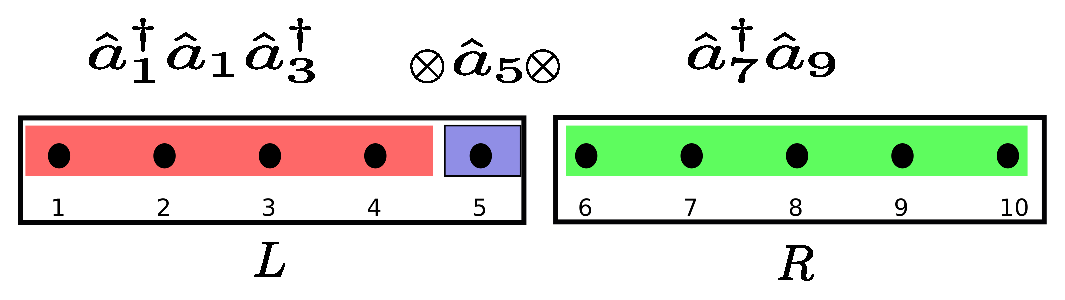
\includegraphics[width=8cm]{operator_split.eps}
  \caption{Evaluation of a three RDM element $\gamma_{1,3,7;1,5,9}$. $\hat{a}_1^\dagger\hat{a}_1\hat{a}^\dagger_3$ is on $\mathcal{S}$, $\hat{a}_5$ is on $\mathcal{D}$, and $\hat{a}^\dagger_7\hat{a}^\dagger_9$ is on $\mathcal{E}$. It belongs to (3,1,2) ``number pattern'' and ($\hat{a}^\dagger\hat{a}\hat{a}^\dagger\hat{a}\hat{a}^\dagger\hat{a}$) ``type pattern''.}
\end{figure}

  After building operators on each block, $\hat{O}^S$, $\hat{O}^D$, $\hat{O}^E$, combine $\hat{O}^S$ and $\hat{O}^D$ into $O^L$, a big left block $\mathcal{S}\otimes \mathcal{D}$. (Combining $\mathcal{E}$ and $\mathcal{D}$ only for RDM calcualtions is also feasible.) The $\mathcal{E}$ is the right block.
  RDM element $\gamma = \sum_{l,r}\sum_{l',r'} c_{l,r} O^{L}_{l,l'} O^R_{r,r'}c_{l',r'}$ , with $\ket{\Psi} = c_{l,r}\ket{l}\ket{r}$, can be computed in two step. (1) $X_{r,r'} = \sum_{l}\sum_{l'} c_{l,r} O^{l,l'} c_{l',r'}$. (2) $\gamma = \sum_{r,r'} X_{r,r'} O^R_{r,r'}$.
  The reason for contracting wave function with $O^L$ first is that the dimension of $O^L$ is $4M$ while the dimension of $O^R$ is $M$.
  The number of operation required for forming X is $O(k^{N+1}M^3)$ and that for dot product between $X$ and $O^R$ is $O(k^{2N}M^2)$. 
  The computations for N-RDM are $O(k^{N+1}M^3+k^{2N}M^2)$.




  %The types of operators on different blocks are also determined automatically. In N-RDM, $N$ $\hat{a}^\dagger$ and $N$ $\hat{a}$ form strings with different orders. They represent different type of $O_{LR}$.
  %The strings are partitioned into three parts according to number of operators in different blocks. This process forms 'patterns' (combinations of different type operators) for the RDM calculations. For exampke, in 2-RDM, for $\hat{a}^\dagger_i\hat{a}^\dagger_j\hat{a}_k\hat{a}_l (i\le j\le k\le l)$ type operators with number of indices partition 2-1-1, all $\hat{a}^\dagger_i\hat{a}^\dagger_j (i\le j)$ operators on $\mathcal{S}$ should be combined with each of $\hat{a}_l$ operators on $\mathcal{E}$ and the only one of $\hat{a}_k$ operator on $\mathcal{D}$. 
  %In order to build operators and corresponding intermedaite ($X$ or $Y$) and to reuse them, operators on $\mathcal{S}$ or $\mathcal{E}$ need to be precomputed and stored. Then do a loop over them. And operators on another block could be built on the fly. 

With above process, an expectation value like $\braket{\hat{a}^\dagger_0\hat{a}^\dagger_1\hat{a}_2\hat{a}_3}$ is obtained. For a non-spinadapted DMRG algrithm ( the operators in not a spin tensor), we can get the value of $\gamma_{0,1,3,2}$ by permuting $ \hat{a}_2$ and $\hat{a}_3$. For spinadapted DMRG operators, what we get is a set of $\braket{\hat{a}^\dagger_0\hat{a}^\dagger_1\hat{a}_2\hat{a}_3}$  values. They are $\braket{\{[(\hat{a}^\dagger_0\hat{a}^\dagger_1)^{S_1}_{\mathcal{S}}(\hat{a}_2)_{\mathcal{D}}]^{S_2}(\hat{a}_3)_{\mathcal{E}}\}^{S_3}}$ with different spins $S_1$, $S_2$, $S_3$. The spin tensors can be expanded as linear combination of spin orbital operators and linear equations are formed for spin orbital RDM elements. With spin embeding, expectation values of all spin tensors with non-zero spin are zero, significantly decrease the number of expectation values to compute. The coefficiencies for these linear equations are the same for the operators in the same pattern and can be generated autmaticaly and be reused. Computation cost for this process is not related the bond dimension, M and is ignorable compared to other parts.
%The spin orbital Nth order RDM elements, solutions of these linear equations, has $(N!)^2$ fold permutation symmetry, much more than correponding spin-averaged RDM's $N!$ fold permuation symmetry, even though the number of element is $2^{2N}$ time of that in spin-averaged RDM.

The computation of 4RDM, which is needed in DMRG-NEVPT is $O(k^8M^2+k^5M^3)$, much higher than that of DMRG optimization. Therefore, the bond dimension of MPS in 4RDM calculations is limited. With the same bond dimension, MPS from a ``reverse schedule'' sweep is usually better optimized that MPS from standard sweep schedule, in which the bond dimension is increased. All of our NEVPT calculations use MPS optmized through ``reverse schedule''.

%The one-particle and two-particle density matrix is defined in this way
%
%\begin{equation}
%\gamma_{i,j}= \sum_\sigma\bra{\Psi}a^\dagger_{i,\sigma}a_{j,\sigma}\ket{\Psi}
%\end{equation}
%\begin{equation}
%\gamma_{i,j,k,l}=\sum_{\sigma,\tau} \bra{\Psi}a^\dagger_{i,\sigma}a^\dagger_{j,\tau}a_{k,\tau}a_{l,\sigma}\ket{\Psi}
%\end{equation}
%
%\subsection{High order particle density matrix}
%Three and four particle density matrix can be used to do multi-reference perturbation calculations. Large number of operators needed in the calculations, high computation scaling and complex spin coupling make the higher order particle density matrix not trivial. We implemented a module to compute different order particle density matrix. It can do loops among different types of operators, pick the non-redundant elements and form linear equations between spin coupling elements and spin average particle density matrix elements, automatically. 
%
%There are $k^8$ elements in four particle density matrix. A trivial way to compute is to compute $<\hat{O}>$($\hat{O}$ has eight indexes) one by one. The scaling is $k^8M^3$. Using intermediate like $\hat{O}[L]\ket{\Psi}$, $\bra{\Psi}\hat{O}[R]$,( a citation), the computation requirement is $O(k^8M^2+k^5M^3)$. It is similar for three particle density matrix. 
%
%Generally, $\hat{O}[L]$ and $\hat{O}[R]$ in four particle density matrix have four indexes. The number of them is $O(k^4)$. It is 
%impossible to store them in the memory in a realistic calculation. They can be divided into different types, based on the number of 
%creation or annihilation operators. Only certain combinations of types of $\hat{O}[L]$ and $\hat{O}[R]$ can have non zero expect value and 
%contribute to results of particle density matrix. One of these combinations are computed at a time. Memory requirement is smaller. 
%
%(Algorithm loops here?)
%
